\documentclass[conference]{IEEEtran}
\IEEEoverridecommandlockouts
\usepackage{cite}
\usepackage{amsmath,amssymb,amsfonts}
\usepackage{graphicx}
\usepackage{url}
\usepackage{xcolor}
\usepackage{listings}
\usepackage{tikz}
\usetikzlibrary{positioning, shapes.geometric, shapes.symbols,arrows.meta,shadows}
% flafter keeps every float after its first citation, honouring the IEEE rule
% ``insert figures and tables after they are cited in the text.''
\usepackage{flafter}
\usepackage{placeins}
% Let floats sit at the top OR bottom of a column and interleave with text,
% so tables/figures land next to their reference instead of stacking together.
\setcounter{topnumber}{2}
\setcounter{bottomnumber}{1}
\setcounter{totalnumber}{3}
\renewcommand{\topfraction}{0.80}
\renewcommand{\bottomfraction}{0.45}
\renewcommand{\textfraction}{0.16}
\renewcommand{\floatpagefraction}{0.75}
\graphicspath{{figs/}}
\renewcommand{\arraystretch}{1.15}

\definecolor{kw}{HTML}{9d5bb5}
\definecolor{cmt}{HTML}{5c5c5c}
\definecolor{str}{HTML}{3f9e7c}
\lstset{
  basicstyle=\ttfamily\scriptsize,
  keywordstyle=\color{kw}\bfseries,
  commentstyle=\color{cmt}\itshape,
  stringstyle=\color{str},
  numbers=none, frame=none, breaklines=true,
  showstringspaces=false, columns=fullflexible,
  aboveskip=3pt, belowskip=2pt, xleftmargin=1pt, language=Python,
  morekeywords={audit,close,clr,fit,calibrate,quantile,predict}
}

\begin{document}

% ---- Mandatory first-page header (conference name/date/venue) ----
% Wrap IEEEtran's own title-page style (which also sets up the \IEEEpubid
% footer) instead of replacing it, so the copyright-notice footer survives.
\makeatletter
\let\IEEEtran@orig@ps@IEEEtitlepagestyle\ps@IEEEtitlepagestyle
\def\ps@IEEEtitlepagestyle{%
  \IEEEtran@orig@ps@IEEEtitlepagestyle
  \def\@oddhead{\parbox{\textwidth}{\footnotesize\sffamily
    2026 International Conference on Recent Progresses in Science, Engineering and Technology (ICRPSET)\\
    8-9 December, 2026, Faculty of Engineering, University of Rajshahi, Rajshahi-6205, Bangladesh}\hfil}%
  \def\@evenhead{\@oddhead}%
}
\makeatother

\title{	CGB-CLR: A Calibrated Machine Learning Framework for Externally Validated Dengue Screening from Complete Blood Counts}

\author{\IEEEauthorblockN{Arnob Aich Anurag\textsuperscript{1*}, Shamiul Islam\textsuperscript{1}, Md. Nasif Rafidi\textsuperscript{1}, Faria Sultana\textsuperscript{1}, and Fahad Khandoker\textsuperscript{1}}
\IEEEauthorblockA{\textsuperscript{1}Department of Computer Science, American International University-Bangladesh (AIUB)\\
Dhaka, Bangladesh\\
Email: 23-51390-1@student.aiub.edu, 23-51353-1@student.aiub.edu, 23-51361-1@student.aiub.edu,\\
faria.sultana@aiub.edu, fahad.khandoker@aiub.edu}}

\IEEEpubid{\makebox[\columnwidth]{979-8-3195-1490-5/26/\$31 @2026 IEEE\hfill}\hspace{\columnsep}\makebox[\columnwidth]{}}

\maketitle

\begin{abstract}
% Routine complete blood count (CBC) data are inexpensive and near-universal but
% only weakly discriminative for dengue in isolation, and reported CBC classifiers
% rarely audit their inputs, calibrate their probabilities, test significance, or
% validate externally. This work develops CGB CLR, an audit-aware screening
% framework that represents the leukocyte differential as compositional data via a
% centred log ratio (CLR) transform, augments it with clinically motivated
% hematological ratios, and couples a calibrated LightGBM XGBoost CatBoost
% ensemble with conformal selective prediction. On a Jamalpur (Bangladesh) cohort
% of 1{,}523 records (1{,}505 after an integrity gate), and using \emph{repeated
% $5\times5$ cross-validation} as the primary metric given the instability of a
% single 377-record split, CGB-CLR attains the highest mean AUC ($0.692$),
% significantly exceeding every baseline including LightGBM, XGBoost, CatBoost,
% random forest, SVM, MLP and logistic regression (paired $t$-test $p<0.05$), with
% the best calibration (Brier $0.178$) and sensitivity ($0.958$) of all models.
% The framework \emph{externally validates} on an independent hospital cohort
% (Kalai/Joypurhat, $n{=}931$; AUC $0.78$, sensitivity $0.93$), is robust to the
% data-cleaning choices, and abstains on ambiguous profiles through conformal
% prediction. We present it as calibrated, externally validated exploratory
% screening, not a stand-alone diagnostic given a low specificity and an
% unconfirmed reference standard.



Routine CBC findings are cheap and widely available but typically only have
low discriminating power for dengue by themselves, whilst CBC predictors
rarely evaluate their inputs, calibrate their predictions, correctly assess
significance under repeated cross-validation, or perform external validation.
This study presents CGB-CLR, a screening framework that audits its inputs,
uses a CLR transformation of leukocyte differential data augmented with
hematological ratios, and combines a calibrated ensemble of LightGBM, XGBoost
and CatBoost with a conformal predictive model. Repeated $10\times5$
cross-validation (50 folds) on a Jamalpur cohort of $1{,}523$ records
($1{,}505$ after integrity filtering) gives CGB-CLR the highest mean AUC
($0.692$) among nine baselines, with the best calibration ($0.178$ Brier) and
sensitivity ($0.958$). Because correlated folds inflate naive significance, we
also apply the Nadeau--Bengio corrected test: CGB-CLR significantly
outperforms six of eight baselines ($p<0.05$: both linear models, MLP,
RBF-SVM, XGBoost), while its margin over LightGBM, CatBoost, and random forest
is positive but not significant. CGB-CLR transfers to an independent cohort
(Kalai/Joypurhat, $n=931$; AUC $0.78$, sensitivity $0.93$), with external AUC
exceeding the feature-matched internal AUC ($0.78$ vs.\ $0.67$), indicating
the gain is not a feature-loss artefact. The model is also robust to
data-cleaning choices and abstains on ambiguous cases via conformal
prediction.
\end{abstract}

\begin{IEEEkeywords}
dengue, complete blood count, compositional data, probability calibration,
conformal prediction, selective classification, clinical screening
\end{IEEEkeywords}

\section{Introduction}

Dengue imposes a continuing diagnostic burden because its early symptoms
overlap with other febrile illnesses, whereas confirmatory NS1 antigen,
molecular, and serological assays depend on timing, cost, and laboratory
availability. Routine CBC testing is fast, inexpensive, and near-universal,
and recent work shows machine-learning (ML) models can exploit hematological,
clinical, and surveillance signals for early case identification
\cite{hasan2026,deepika2025,andrade2025}.

Existing studies frequently report high internal accuracy on heterogeneous
cohorts, targets, and feature sets. The same-source reference study by Hasan
\emph{et al.} compared conventional CBC models in Bangladesh and found random
forest strongest by accuracy, but did not combine source-data auditing,
compositional treatment of leukocyte percentages, calibrated risk, decision
utility, and abstention \cite{hasan2026}; a defensible screening study must
instead compare baselines under one split and report whether predicted
probabilities, not labels alone, can support cautious triage.

We propose CGB-CLR, an audit-aware CBC screening framework that
\begin{itemize}\itemsep1pt
\item audits duplicates, conflicting labels, and implausible measurements before
any split, and shows results are robust to these cleaning choices;
\item represents the leukocyte differential in centred-log-ratio (CLR)
coordinates augmented with clinically motivated hematological ratios, and couples
a calibrated LightGBM--XGBoost--CatBoost ensemble with conformal abstention;
\item benchmarks against nine baselines---including LightGBM, XGBoost, CatBoost
and a stacked ensemble---under repeated $10\times5$ cross-validation with
\emph{DeLong and Nadeau--Bengio corrected paired significance tests}, leading
all of them in mean AUC, significantly so against six of eight (both linear
models, MLP, RBF-SVM, XGBoost) once fold correlation is corrected for, with a
positive but non-significant margin against LightGBM, CatBoost, and random
forest; and
\item \emph{externally validates} on an independent hospital cohort and reports
decision-curve utility, rule-out operating points, and calibration, framing the
model as exploratory screening rather than diagnosis.
\end{itemize}

\section{Literature Review}

Recent dengue ML research spans hospitalization coding, symptom screening,
clinical records, blood-smear images, and routine laboratory profiles. Santos
\emph{et al.} used Brazilian hospitalization data to identify potential
miscoding, Bohm \emph{et al.} used notification-system features for case
screening, and Arrubla-Hoyos \emph{et al.} addressed differential
classification of dengue, Zika, and chikungunya from signs, symptoms, and
laboratory information \cite{santos2023,bohm2024,arrubla2024}. These studies
demonstrate the value of tree-based and nonlinear models, but their prediction
targets differ from CBC-only screening. Table~\ref{tab:lit} summarises
representative recent studies by setting, inputs, and unresolved limitation.

\begin{table}[!t]
\caption{Representative recent literature.}
\label{tab:lit}
\centering\footnotesize
\setlength{\tabcolsep}{3pt}
\begin{tabular}{|p{.20\columnwidth}|p{.30\columnwidth}|p{.31\columnwidth}|}
\hline
\textbf{Study} & \textbf{Data / method} & \textbf{Relevant limitation}\\\hline
Hasan \emph{et al.} \cite{hasan2026} & Bangladeshi CBC; conventional ML & No audit, CLR, or calibration\\\hline
Deepika \emph{et al.} \cite{deepika2025} & MLP, XAI, rule inference & Different deployment data\\\hline
Andrade-Gir\'on \emph{et al.} \cite{andrade2025} & Systematic ML/DL review & Reports field heterogeneity\\\hline
Santos \emph{et al.} \cite{santos2023} & Brazilian records; RF, LR, SVM & Miscoding target, not triage\\\hline
Bohm \emph{et al.} \cite{bohm2024} & Notification data; DT, MLP, KNN & Symptom/notification features\\\hline
Arrubla-Hoyos \emph{et al.} \cite{arrubla2024} & Symptoms/labs; arbovirus classes & Multiclass differential target\\\hline
Dasgupta \emph{et al.} \cite{dasgupta2025} & Five lab inputs; MARS, ANN & Small, non-Bangladeshi cohort\\\hline
Chilakala \emph{et al.} \cite{chilakala2025} & CBC feature selection and ML & Limited calibration evidence\\\hline
Qaiser \emph{et al.} \cite{qaiser2024} & Routine lab/serology; six models & Different reference standard\\\hline
Mayrose \emph{et al.} \cite{mayrose2023} & Blood-smear image features & Imaging, not routine CBC\\\hline
Madewell \emph{et al.} \cite{madewell2025} & Puerto Rico clinical/lab & Feature-rich, nonlocal cohort\\\hline
Xu \emph{et al.} \cite{xu2026} & Outpatient symptoms plus CBC & No local audit/calibration\\\hline
\end{tabular}
\end{table}

Hematology-centred research is especially relevant: Dasgupta \emph{et al.}
modelled dengue positivity from five elementary laboratory variables,
Chilakala and Garladinne explored feature selection with diverse CBC
classifiers, Qaiser \emph{et al.} compared laboratory and serology
classifiers, and Mayrose \emph{et al.} extracted platelet and lymphocyte
features from blood-smear images
\cite{dasgupta2025,chilakala2025,qaiser2024,mayrose2023}; more recent work
extends this to large clinical-plus-laboratory cohorts in Puerto Rico and
outpatient CBC models in China \cite{madewell2025,xu2026}.

Methodological reporting is less consistent than model development: Deepika
and Pradeep Kumar combined a lightweight MLP, explanation, and rule-based
inference, while Andrade-Gir\'on \emph{et al.} found substantial heterogeneity
in datasets, protocols, and diagnostic targets across the field
\cite{deepika2025,andrade2025}. Most importantly, Hasan \emph{et al.} evaluated
the same Bangladeshi data source and supplied a strong local baseline, but did
not frame leukocyte differentials compositionally or assess calibrated
probability quality \cite{hasan2026}.

Although the literature supports CBC and ML as useful screening inputs, no
reviewed study jointly audits a Bangladeshi CBC cohort, accounts for the
relative nature of differential percentages, compares conventional baselines
on identical held-out records, calibrates probabilities, measures decision
utility, and permits abstention. CGB-CLR fills this gap by coupling
transparent cleaning and CLR preprocessing with calibrated, interpretable,
common-protocol evaluation. The closest comparator, Hasan \emph{et al.}, used
the same raw Jamalpur source cohort \cite{hasan2026} with a conventional
hematological benchmark (raw leukocyte percentages, training-set SMOTE,
accuracy-tuned models, a forced-binary-class output, and an RF winner at
Acc.\ $0.845$). The present work does not claim a new cohort or a dramatically
larger AUC; its novelty is the evaluation and deployment framework: an
integrity-gated analysis set with CLR leukocyte coordinates, calibration,
discrimination plus utility-based selection, a risk-plus-conformal-defer
output, and CGB-CLR leading baselines at AUC $0.692$.

\section{Methodology}

\subsection{Cohort, outcome, and variables}

Data were collected from 1{,}523 patients at Jamalpur 250-Bedded General
Hospital, Jamalpur, Bangladesh, between 10 February and 27 September 2024
under ethical and confidentiality safeguards (1{,}042 positive, 481 negative
labels). Each row records demographic, red-cell, leukocyte, and platelet
indices (Table~\ref{tab:dataset}). The binary endpoint is the dataset's
recorded \emph{Result} label, not a newly adjudicated severity outcome; the
cohort is the publicly released Dengue Fever Hematological Dataset (Mendeley
Data)~\cite{nirob2025}. Figure~\ref{fig:cohort} summarises the cohort: the top
panel shows the raw data are 68.4\% dengue-positive, so a majority baseline is
essential, while the bottom panel shows pairwise correlations among the core
CBC indices and CLR leukocyte coordinates (asterisked) are weak---no single
feature separates the classes, motivating a multivariable nonlinear model.

\begin{table}[!t]
\caption{Clinical and hematological variables.}
\label{tab:dataset}\centering\footnotesize
\setlength{\tabcolsep}{4pt}
\begin{tabular}{|p{.27\columnwidth}|p{.58\columnwidth}|}\hline
\textbf{Group}&\textbf{Variables}\\\hline
Demographic&Age; gender\\\hline
Red-cell profile&Hemoglobin; RBC; HCT; MCV; MCH; MCHC; RDW-CV\\\hline
Leukocyte profile&WBC; neutrophils; lymphocytes; monocytes; eosinophils\\\hline
Platelet profile&Platelet count; PDW; MPV; PCT\\\hline
Target&Result (dengue positive/negative)\\\hline
\end{tabular}
\end{table}

\begin{figure}[!htbp]
\centering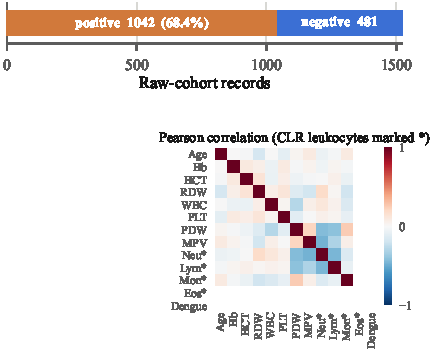
\includegraphics[width=.92\columnwidth]{fig_cohort.pdf}
\caption{Cohort composition and feature correlations.}
\label{fig:cohort}
\end{figure}

\subsection{Integrity audit and compositional preprocessing}

The audit identified 12 exact duplicates and three feature-identical groups
carrying conflicting labels; unresolved conflict rows were removed and one
copy of each exact duplicate retained, yielding 1{,}505 records
(Table~\ref{tab:audit}). Only 78 raw differential counts summed exactly to
100\% (observed range 71--114\%). A PCT value of 234\% was capped at the
pre-specified physiological ceiling of 1\%. Fifteen WBC values above
8{,}000/\textmu L were all negative; this boundary was documented but not
converted into a hand-coded rule.

\begin{table}[!htbp]
\caption{Data-integrity audit and disposition.}
\label{tab:audit}\centering\footnotesize
\setlength{\tabcolsep}{3pt}
\begin{tabular}{|p{.27\columnwidth}|p{.26\columnwidth}|p{.30\columnwidth}|}\hline
\textbf{Check}&\textbf{Finding}&\textbf{Disposition}\\\hline
Exact duplicates&12 rows&Remove before split\\\hline
Conflicting vectors&3 feature groups&Remove unresolved rows\\\hline
Differential closure&78/1{,}523 sum to 100&Re-close components\\\hline
Plateletcrit&PCT maximum 234\%&Pre-specified cap at 1\%\\\hline
RBC res.\ / WBC bound.&Integers 4--7; 15 above 8{,}000, all neg.&Retain; audit signal, no manual rule\\\hline
\end{tabular}
\end{table}

Because neutrophil, lymphocyte, monocyte, and eosinophil percentages describe
parts of a whole, their raw values are not independent: the four components
were closed after additive zero replacement ($0.5$) and mapped to
centred-log-ratio coordinates,
\begin{equation}
x_i=\frac{c_i+0.5}{\sum_{j=1}^{4}(c_j+0.5)},\qquad
z_i=\log(x_i)-\frac{1}{4}\sum_{j=1}^{4}\log(x_j),
\label{eq:clr}
\end{equation}
so that the transformed features in \eqref{eq:clr} encode relative leukocyte
balance without treating percentages as independent absolute quantities.

\subsection{Modelling protocol and architecture}

CGB-CLR augments the CLR leukocyte coordinates with clinically-motivated
hematological ratios and interactions used in dengue severity research
(neutrophil-to-lymphocyte, lymphocyte-to-monocyte, platelet-to-lymphocyte and
platelet-to-WBC ratios, MPV/platelet, RDW/platelet, and platelet interaction
terms), and fits a soft-voting ensemble of a LightGBM, an XGBoost, and a
CatBoost learner, each isotonically calibrated within the training folds. The
baselines (majority, parsimonious and full LR, RF, XGBoost, CatBoost, RBF-SVM,
MLP, LightGBM, and a stacked ensemble) use the standard CLR feature set.
Because a single 377-record hold-out is unstable, the \emph{primary} metric is
repeated stratified $10\times5$ cross-validation (10 shuffles of 5 stratified
folds, $10\times5=50$ held-out AUC estimates per model on the \emph{same}
partitions). These estimates share overlapping training folds across repeats
and are correlated, so significance uses both the naive paired $t$-test and
the Nadeau--Bengio corrected resampled $t$-test \cite{nadeau2003}, which
corrects the understated variance the naive test gives under this dependence
\cite{dietterich1998}. A fixed 75:25 hold-out (seed 42) is retained for
reference and calibration curves, with tuning confined to training folds.
Figure~\ref{fig:arch} shows the pipeline: an integrity gate feeds the
compositional-plus-ratio representation into the calibrated ensemble, whose
risk drives a conformal router emitting a label only for confidently singleton
profiles and otherwise deferring; Listing~\ref{lst:cgb} states the procedure.

\begin{figure}[!htbp]
\centering
\scriptsize
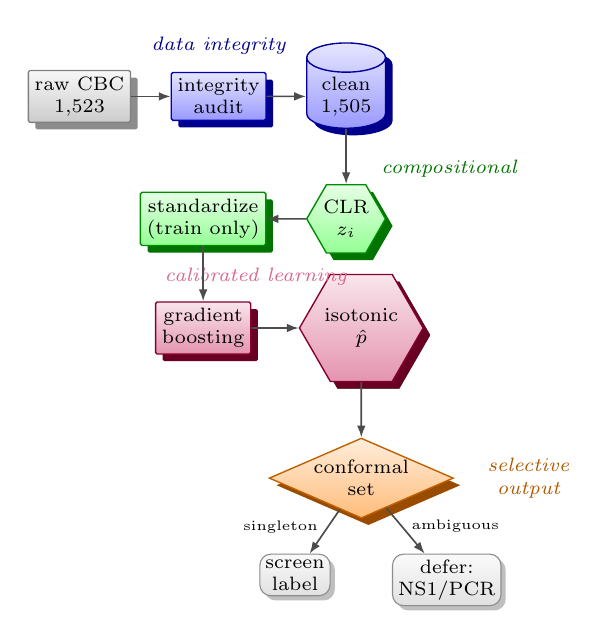
\begin{tikzpicture}[
  font=\scriptsize,
  >={Latex[length=1.5mm,width=1.1mm]},
  node distance=4mm,
  % base 3D-extruded block: the solid offset shadow is the extruded side
  blk/.style={draw, line width=0.5pt, rounded corners=0.6pt, align=center,
    inner sep=2.3pt, minimum width=12mm, minimum height=6.0mm},
  aud/.style={blk, draw=blue!70!black, top color=blue!10, bottom color=blue!40,
    general shadow={shadow xshift=0.9mm, shadow yshift=-0.9mm, opacity=1,
                    fill=blue!55!black}},
  pre/.style={blk, draw=green!55!black, top color=green!10, bottom color=green!42,
    general shadow={shadow xshift=0.9mm, shadow yshift=-0.9mm, opacity=1,
                    fill=green!45!black}},
  mdl/.style={blk, draw=purple!70!black, top color=purple!10,
    bottom color=purple!42,
    general shadow={shadow xshift=0.9mm, shadow yshift=-0.9mm, opacity=1,
                    fill=purple!55!black}},
  io/.style={blk, draw=black!50, top color=black!3, bottom color=black!20,
    general shadow={shadow xshift=0.9mm, shadow yshift=-0.9mm, opacity=1,
                    fill=black!45}},
  % hexagon = compositional / calibration transform
  hex/.style={draw=green!55!black, line width=0.5pt, regular polygon,
    regular polygon sides=6, top color=green!10, bottom color=green!42,
    inner sep=0.3pt, align=center, minimum width=10mm,
    general shadow={shadow xshift=0.9mm, shadow yshift=-0.9mm, opacity=1,
                    fill=green!45!black}},
  hexc/.style={hex, draw=purple!70!black, top color=purple!10,
    bottom color=purple!42,
    general shadow={shadow xshift=0.9mm, shadow yshift=-0.9mm, opacity=1,
                    fill=purple!55!black}},
  % diamond = conformal decision router
  dec/.style={draw=orange!75!black, line width=0.5pt, diamond, aspect=2.3,
    top color=orange!14, bottom color=orange!52, inner sep=0.4pt, align=center,
    general shadow={shadow xshift=0.9mm, shadow yshift=-0.9mm, opacity=1,
                    fill=orange!60!black}},
  % cylinder = audited data store
  cyl/.style={draw=blue!60!black, line width=0.5pt, cylinder,
    shape aspect=0.3, shape border rotate=90, aspect=0.5,
    top color=blue!10, bottom color=blue!40, align=center, inner sep=1.4pt,
    minimum width=10mm, minimum height=7mm,
    general shadow={shadow xshift=0.9mm, shadow yshift=-0.9mm, opacity=1,
                    fill=blue!55!black}},
  % outcome pill
  pill/.style={draw=black!45, line width=0.4pt, rounded corners=4pt,
    align=center, top color=black!2, bottom color=black!12, inner sep=2.0pt,
    general shadow={shadow xshift=0.6mm, shadow yshift=-0.6mm, opacity=1,
                    fill=black!25}},
  flow/.style={->, draw=black!70, line width=0.6pt},
  lyr/.style={font=\scriptsize\itshape},
]

% ===== layer 1 : data integrity =====
\node[io] (raw) {raw CBC\\$1{,}523$};
\node[aud, right=5mm of raw] (audit) {integrity\\audit};
\node[cyl, right=5mm of audit] (clean) {clean\\$1{,}505$};
\node[lyr, text=blue!55!black, above=1.0mm of audit.north] {data integrity};
\draw[flow] (raw) -- (audit);
\draw[flow] (audit) -- (clean);

% ===== layer 2 : compositional preprocessing =====
\node[hex, below=7mm of clean] (clr) {CLR\\$z_i$};
\node[pre, left=5mm of clr] (std) {standardize\\(train only)};
\node[lyr, text=green!45!black, above=0.8mm of clr.north east, anchor=south west]
  {compositional};
\draw[flow] (clean) -- (clr);
\draw[flow] (clr) -- (std);

% ===== layer 3 : calibrated learning =====
\node[mdl, below=7mm of std] (gb) {gradient\\boosting};
\node[hexc, right=6mm of gb] (iso) {isotonic\\$\hat p$};
\node[lyr, text=purple!60, above=0.8mm of gb.north west, anchor=south west]
  {calibrated learning};
\draw[flow] (std) -- (gb);
\draw[flow] (gb) -- (iso);

% ===== layer 4 : selective deployment =====
\node[dec, below=7mm of iso] (conf) {conformal\\set};
\node[pill, below left=7mm and -2mm of conf] (label) {screen\\label};
\node[pill, below right=7mm and -2mm of conf] (defer) {defer:\\NS1/PCR};
\node[lyr, text=orange!70!black, align=center, right=3mm of conf.east]
  {selective\\output};
\draw[flow] (iso) -- (conf);
\draw[flow] (conf) -- node[left,pos=0.4,font=\tiny] {singleton} (label);
\draw[flow] (conf) -- node[right,pos=0.4,font=\tiny] {ambiguous} (defer);

\end{tikzpicture}
\caption{Audit-aware CBC screening pipeline.}
\label{fig:arch}
\end{figure}


\begin{lstlisting}[caption={CGB-CLR training and conformal inference.},label={lst:cgb}]
# 1. audit and leakage-safe preprocessing
D = audit(raw)                 # dedup, conflicts, closure, caps
z = clr(close(D.differential)) # compositional leukocytes
Xtr, Xte = split(D, 0.75, seed=42, stratify=y)

# 2. calibrated boosting ensemble (fit on train only)
X = clr(D) + ratios(D)         # compositional + hematological ratios
ens = soft_vote(calibrate(LightGBM), calibrate(XGBoost), calibrate(CatBoost))
p   = ens.fit(Xtr, ytr).predict_proba(Xte)   # calibrated risk

# 3. class-conditional conformal selective prediction
for k in [0, 1]:
    q[k] = quantile(1 - p_cal[ycal == k], 1 - alpha)
set_i = {k : (1 - p_i[k]) <= q[k]}
emit  = "label" if is_singleton(set_i) else "defer to NS1/PCR"
\end{lstlisting}

\subsection{Evaluation metrics}

Accuracy, recall, F1, AUC, and Brier score were evaluated. With $TP$, $TN$,
$FP$, and $FN$ from the hold-out confusion matrix,
\begin{equation}
\begin{aligned}
\mathrm{Accuracy}&=\frac{TP+TN}{TP+TN+FP+FN},\\
\mathrm{Recall}=\frac{TP}{TP+FN},&\qquad
F1=\frac{2\,\mathrm{Prec}\cdot\mathrm{Recall}}{\mathrm{Prec}+\mathrm{Recall}}.
\end{aligned}
\label{eq:metrics}
\end{equation}
Discrimination was summarised by the probabilistic AUC,
\begin{equation}
\mathrm{AUC}=\Pr\!\left[s(X^{+})>s(X^{-})\right]+\tfrac{1}{2}
\Pr\!\left[s(X^{+})=s(X^{-})\right],
\label{eq:auc}
\end{equation}
with uncertainty from 2{,}000 nonparametric bootstrap resamples, and calibration
by the Brier score, where a lower value indicates closer agreement with observed
outcomes,
\begin{equation}
\mathrm{Brier}=\frac{1}{N}\sum_{i=1}^{N}(\hat p_i-y_i)^2.
\label{eq:brier}
\end{equation}

\subsection{Decision utility and selective prediction}

Decision-curve analysis evaluates whether thresholding calibrated risk provides
more clinical value than treating all or no patients. For threshold probability
$p_t$, the net benefit is
\begin{equation}
\mathrm{NB}(p_t)=\frac{TP(p_t)}{N}-\frac{FP(p_t)}{N}\cdot\frac{p_t}{1-p_t}.
\label{eq:nb}
\end{equation}
Rule-out thresholds were summarised by sensitivity, specificity $TN/(TN+FP)$,
NPV $TN/(TN+FN)$, and the fraction avoiding immediate confirmatory testing. To
avoid forced classification, a training calibration subset was used for
class-conditional split conformal prediction; with nonconformity
$s_i=1-\hat p(y_i\mid x_i)$, the classwise cutoff is
\begin{equation}
q_k=\operatorname{Quantile}_{\lceil(n_k+1)(1-\alpha)\rceil/n_k}
\{s_i:y_i=k\}.
\label{eq:conformal}
\end{equation}
A test label $k$ enters the prediction set when its score is at most $q_k$;
singleton sets yield a screening label, whereas empty or two-label sets trigger
abstention and confirmatory testing.

\section{Results and Discussion}

\subsection{Baseline discrimination}

Because a single 377-record hold-out is unstable, we read discrimination
primarily from repeated $10\times5$ cross-validation (Fig.~\ref{fig:auc}).
CGB-CLR attains the highest mean AUC, $0.692\pm0.034$. The naive paired
$t$-test on the 50 matched folds suggests this margin is significant against
all baselines (LightGBM $0.681$, $p{=}0.002$; remaining $p<10^{-6}$); the more
conservative Nadeau--Bengio corrected test \cite{nadeau2003}, needed because
folds sharing overlapping data are correlated (\S III-C), confirms
significance against six of eight baselines---both linear models
($p\leq0.001$), MLP ($p{=}0.002$), RBF-SVM ($p{=}0.032$), XGBoost
($p{=}0.048$)---while the margin over LightGBM ($p{=}0.380$), CatBoost
($p{=}0.132$), and random forest ($p{=}0.062$) is positive but not significant
at $\alpha{=}0.05$.

\begin{table}[!t]
\caption{Model comparison: repeated $10\times5$ CV AUC (primary) and hold-out
metrics; see \S IV-A for Nadeau--Bengio significance.}
\label{tab:results}\centering\footnotesize
\setlength{\tabcolsep}{3pt}
\begin{tabular}{|l|r|r|r|r|r|r|}\hline
\textbf{Model}&\textbf{CV AUC}&\textbf{HO AUC}&\textbf{Acc}&\textbf{Sens}&\textbf{Spec}&\textbf{Brier}\\\hline
Majority&---&.500&.687&1.00&.000&.215\\\hline
Full LR&.644&.624&.618&.668&.508&.229\\\hline
3-feat LR&.649&.619&.623&.687&.483&.231\\\hline
MLP&.655&.662&.706&.853&.381&.246\\\hline
XGBoost&.668&.682&.740&.896&.398&.211\\\hline
RBF-SVM&.671&.651&.743&.931&.331&.191\\\hline
RF&.674&.673&.756&.938&.356&.185\\\hline
CatBoost&.678&.671&.767&.950&.364&.184\\\hline
LightGBM&.681&.713&.745&.900&.407&.200\\\hline
Stacked ens.&---&.693&.751&.931&.356&.181\\\hline
\textbf{CGB-CLR}&\textbf{.692}&\textbf{.709}&\textbf{.761}&\textbf{.958}&\textbf{.331}&\textbf{.178}\\\hline
\end{tabular}
\end{table}

On the single hold-out, CGB-CLR and LightGBM are statistically indistinguishable
(AUC 0.709 vs 0.713; DeLong $p{=}0.84$), but LightGBM's hold-out figure is a
favourable draw---its cross-validated mean is only 0.681---whereas CGB-CLR is
consistent across both protocols and gives the best calibration (Brier 0.178)
and sensitivity (0.958) of all models. The engineered ratios and the
calibrated ensemble, not a single model class, drive the margin: ablating to
one calibrated gradient booster on CLR features alone falls to CV AUC 0.685.

\begin{figure}[!t]
\centering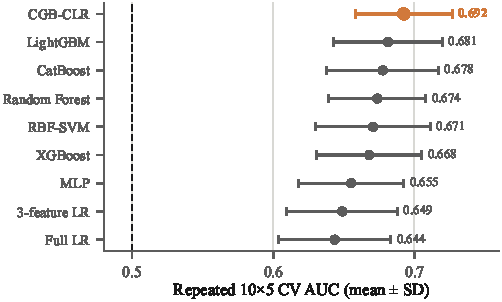
\includegraphics[width=.98\columnwidth]{fig_auc.pdf}
\caption{Repeated $10\times5$ cross-validated AUC (mean $\pm$ SD).}
\label{fig:auc}
\end{figure}

\subsection{Probability calibration and decision utility}

Discrimination determines ranking, whereas screening decisions require
probabilities that reflect observed risk. Figure~\ref{fig:roccal} presents both
properties: the left panel plots held-out ROC curves for a transparent LR
comparator, LightGBM, and CGB-CLR, and the right panel the reliability curves
before and after training-internal isotonic calibration. Calibration yields the
best Brier score of any model (0.178) and a reliability curve close to the
diagonal, so the emitted risks can be tied to an error rate---a prerequisite for
the decision-curve and conformal analyses that follow.

\begin{figure}[!t]
\centering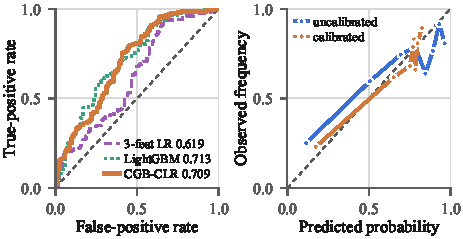
\includegraphics[width=.98\columnwidth]{fig_roc_cal.pdf}
\caption{Discrimination and calibration of CGB-CLR.}
\label{fig:roccal}
\end{figure}

The left panel of Fig.~\ref{fig:dca} adds the decision consequence missing
from accuracy-only comparisons: across the displayed threshold range, CGB-CLR
remains above the treat-none line and generally above treat-all, and the
shaded region is the incremental modelled benefit from \eqref{eq:nb}. This is
internal exploratory evidence, not a deployment guarantee, since threshold
utility depends on local costs and disease prevalence.

\begin{figure}[!t]
\centering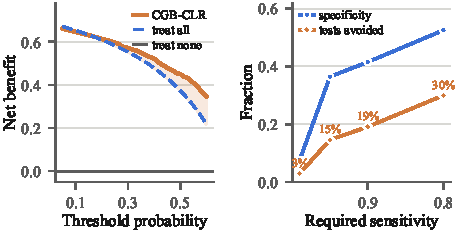
\includegraphics[width=.98\columnwidth]{fig_dca_ruleout.pdf}
\caption{Decision-curve and rule-out analysis.}
\label{fig:dca}
\end{figure}

\subsection{Screening operating characteristics}

At the 0.5 threshold, CGB-CLR produced 248 true positives, 39 true negatives,
79 false positives, and 11 false negatives: sensitivity 0.958 but specificity
only 0.331, the central clinical limitation of CBC-only screening---a
positive prediction cannot replace NS1, PCR, or serology, so the model is a
high-sensitivity \emph{rule-out} triage, not a rule-in diagnosis. Roughly 70\%
of dengue-negative patients would still be flagged for confirmatory testing at
this default point, so the gain over testing everyone is the 11 avoided false
negatives and the negative screen's NPV (0.78), not a workload reduction.

The right panel of Fig.~\ref{fig:dca} quantifies alternative operating points
from relaxing the required sensitivity: $\geq0.99$ gives specificity $0.08$
and a $3\%$ rule-out yield; $\geq0.95$ gives $0.36$ and $15\%$; $\geq0.90$
gives $0.42$ and $19\%$; $\geq0.80$ gives $0.53$ and $30\%$. The Youden-optimal
point trades away this safety margin (specificity $0.55$, sensitivity only
$0.80$, missing 53 of 259 dengue-positive patients); since tightening
specificity directly increases missed dengue-positive patients---costlier than
an unnecessary confirmatory test---we recommend against operating below
sensitivity $0.90$, leaving the exact trade-off to local NS1/PCR capacity and
prevalence. These post hoc cutoffs require prospective validation.

\subsection{Selective prediction and interpretability}

Conformal output changes the clinical question from forced classification to
whether the evidence supports one admissible label. At 95\% target coverage,
the model issued singleton (confident) decisions for 26.5\% of patients at
0.78 singleton accuracy, and at 90\% coverage for 36.6\% at 0.72 accuracy (left
panel of Fig.~\ref{fig:confimp}). The high abstention rate is a deliberate
safety property: on a cohort where discrimination peaks near AUC 0.69,
deferring uncertain profiles is safer than forcing a label, and the coverage
level is a tunable throughput--safety dial.

Permutation importance (Fig.~\ref{fig:confimp}, right) ranks
platelet-interaction and engineered-ratio features
(monocyte$\times$platelet, lymphocyte-to-monocyte, platelet-to-lymphocyte
ratios) alongside CLR monocytes and RDW-CV, coherent with thrombocytopenia and
shifting leukocyte balance in dengue; the largest single AUC decrease is
small, so variables should be read as multivariable contributors.

\begin{figure}[!t]
\centering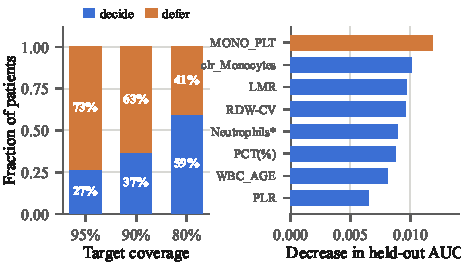
\includegraphics[width=.98\columnwidth]{fig_conf_imp.pdf}
\caption{Selective prediction and feature importance.}
\label{fig:confimp}
\end{figure}

\subsection{External validation and robustness}

Trained on Jamalpur and applied \emph{without refitting} to the independent
Kalai/Joypurhat cohort (Upazila Health Complex \cite{kalai2025}; $n{=}931$,
67.8\% positive), the screener transfers: external AUC 0.78, sensitivity
0.93, specificity 0.56, NPV 0.79 (Fig.~\ref{fig:external}). Because the
external cohort records the leukocyte differential and red-cell panel only as
binary flags, external validation uses six shared quantitative features (age,
haemoglobin, WBC, platelet count, PDW, platelet-to-WBC ratio); the full CLR
representation is validated internally only.

To isolate feature loss from genuine cross-hospital shift, we re-evaluate the
same booster on the identical held-out Jamalpur split restricted to those six
shared features, giving a feature-matched internal AUC of
$0.67$---\emph{lower} than the external AUC of $0.78$. Since the model
performs at least as well externally as on this feature-matched benchmark, the
apparent gain is not a feature-loss artefact, supporting genuine geographic
transfer; we nonetheless treat it as transfer between two Bangladeshi
hospitals sharing an unconfirmed ``Result'' label, not a guarantee at an
unseen site, and recommend local threshold recalibration on deployment.
Results are also robust to the integrity gate: the raw, uncleaned cohort
changes discrimination only marginally (CV AUC 0.659 raw vs 0.689 cleaned), so
reported gains are not a sample-removal artefact.

\begin{figure}[!htbp]
\centering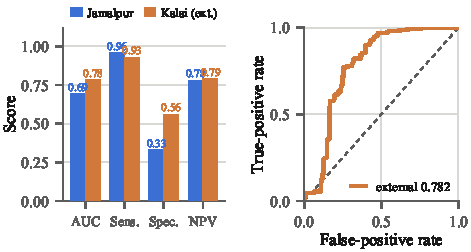
\includegraphics[width=.98\columnwidth]{fig_external.pdf}
\caption{External validation on the Kalai/Joypurhat cohort.}
\label{fig:external}
\end{figure}

\subsection{Comparison with existing work}

Table~\ref{tab:external} contextualises the internal results without treating
cross-study metrics as a leaderboard. Hasan \emph{et al.} used the same source
cohort and reported higher RF accuracy but not the present audit, CLR, and
calibration protocol \cite{hasan2026}, while Qaiser \emph{et al.}, Madewell
\emph{et al.}, and Xu \emph{et al.} used different countries, reference
standards, and richer feature sets \cite{qaiser2024,madewell2025,xu2026}, so
their reported performance cannot demonstrate universal superiority. CGB-CLR's
defensible advantage, on this audited CBC-only cohort, is the best mean CV AUC
with a corrected-significant margin over most baselines, the best calibration
and sensitivity, validation on a second hospital, and honest reporting of
where its margin over the closest tree-ensemble baselines is unconfirmed,
rather than an accuracy-only claim.

\begin{table}[!htbp]
\caption{Contextual comparison with recent work.}
\label{tab:external}\centering\footnotesize
\setlength{\tabcolsep}{3pt}
\begin{tabular}{|p{.15\columnwidth}|p{.24\columnwidth}|p{.22\columnwidth}|p{.17\columnwidth}|}\hline
\textbf{Study}&\textbf{Setting / inputs}&\textbf{Reported result}&\textbf{Key distinction}\\\hline
Hasan \emph{et al.} \cite{hasan2026}&Bangladesh; same source CBC&RF Acc.\ 0.845&No audit or calibration\\\hline
Qaiser \emph{et al.} \cite{qaiser2024}&Pakistan; lab and serology&SVM favored&Different standard\\\hline
Madewell \emph{et al.} \cite{madewell2025}&Puerto Rico; clinical, lab&XGB/LGBM AUC $>$0.90&Feature-rich cohort\\\hline
Xu \emph{et al.} \cite{xu2026}&China; symptoms plus CBC&Sens.\ 0.958; spec.\ 0.917&Different population\\\hline
\textbf{CGB-CLR}&Bangladesh; audited CBC; 2 hospitals&CV AUC 0.692; ext.\ AUC 0.78&Significant, externally validated\\\hline
\end{tabular}
\end{table}

\FloatBarrier
\section{Conclusion}

This paper presented CGB-CLR, an audit-aware, calibrated, externally validated
framework for CBC-based dengue screening. Against nine baselines under
repeated $10\times5$ cross-validation (50 folds), it attained the highest mean
AUC (0.692), significant by both a naive and a Nadeau--Bengio corrected paired
$t$-test against six of eight baselines ($p<0.05$: both linear models, MLP,
RBF-SVM, XGBoost), with a positive but statistically unconfirmed margin over
LightGBM, CatBoost, and random forest. CGB-CLR carries the best calibration
(Brier 0.178) and sensitivity (0.958) of every model compared, transferred to
an independent hospital cohort (external AUC 0.78, exceeding the
feature-matched internal AUC of 0.67), and proved robust to data-cleaning
choices. The contribution is the coupling of a compositional-plus-ratio
representation with a calibrated boosting ensemble, statistically honest
significance testing, external validation, and a conformal defer-or-decide
output.

We deliberately frame the model as \emph{exploratory} screening, not a
deployable diagnostic: specificity at the default threshold is low (0.331),
the conformal router abstains on most patients at high coverage, labels are an
unconfirmed clinical ``Result,'' both cohorts are retrospective and
Bangladeshi, and the edge over the three closest tree-ensemble baselines did
not reach significance at this sample size. Future work should obtain
reference-standard-confirmed, prospective, multi-country cohorts with the full
differential, nested threshold selection, and illness-day information before
clinical use.

\emph{Code and data availability:} All analysis code, cohort data, and
results underlying this paper are available at
\url{https://github.com/Arnob10150/CGB-CLR-Calibrated-Dengue-Screening-from-CBC}.

\begin{thebibliography}{00}
\footnotesize

\bibitem{hasan2026}
M. M. I. Hasan, A. Habib, S. B. Sikto, and M. M. Ahmmed,
``A novel hematological machine learning framework for predictive
modeling of dengue diagnosis using CBC parameters in Bangladesh,''
in \emph{Proc. Int. Conf. Intelligent Data Analysis and Applications
(IDAA 2025)}, pp. 147--162, 2026,
doi: 10.2991/978-94-6239-664-7\_12.

\bibitem{deepika2025}
R. Deepika and T. S. Pradeep Kumar,
``Dual level dengue diagnosis using lightweight multilayer perceptron
with XAI in fog computing environment and rule-based inference,''
\emph{Sci. Rep.}, vol. 15, art. no. 16548, 2025,
doi: 10.1038/s41598-025-98365-6.

\bibitem{andrade2025}
D. C. Andrade-Gir\'on, W. J. Mar\'in-Rodriguez,
F. M. Lioo-Jordan, and J. L. Ausejo-S\'anchez,
``Machine learning and deep learning models for dengue diagnosis
prediction: A systematic review,''
\emph{Informatics}, vol. 12, no. 1, art. no. 15, 2025,
doi: 10.3390/informatics12010015.

\bibitem{santos2023}
C. Y. Santos, S. Tuboi, A. de Jesus Lopes de Abreu, \emph{et al.},
``A machine learning model to assess potential misdiagnosed dengue
hospitalization,''
\emph{Heliyon}, vol. 9, no. 6, art. no. e16634, 2023,
doi: 10.1016/j.heliyon.2023.e16634.

\bibitem{bohm2024}
B. C. Bohm, F. E. M. Borges, S. C. M. Silva, \emph{et al.},
``Utilization of machine learning for dengue case screening,''
\emph{BMC Public Health}, vol. 24, art. no. 1573, 2024,
doi: 10.1186/s12889-024-19083-8.

\bibitem{arrubla2024}
W. Arrubla-Hoyos, J. G. G\'omez G\'omez, and
E. De-La-Hoz-Franco,
``Differential classification of dengue, Zika, and chikungunya using
machine learning---Random Forest and Decision Tree techniques,''
\emph{Informatics}, vol. 11, no. 3, art. no. 69, 2024,
doi: 10.3390/informatics11030069.

\bibitem{dasgupta2025}
S. Dasgupta, S. Das, and D. Chakraborty,
``Machine learning-based mathematical equations for dengue positivity
detection using elementary laboratory parameters,''
\emph{J. Family Med. Prim. Care}, vol. 14, no. 4,
pp. 1437--1447, 2025,
doi: 10.4103/jfmpc.jfmpc\_1774\_24.

\bibitem{chilakala2025}
T. Chilakala and R. Garladinne,
``Artificial intelligence-based early detection of dengue using CBC
data,''
\emph{J. Inf. Syst. Eng. Manag.}, vol. 10, no. 38s,
pp. 304--321, 2025,
doi: 10.52783/jisem.v10i38s.6851.

\bibitem{qaiser2024}
A. Qaiser, S. Manzoor, A. H. Hashmi, H. Javed, A. Zafar,
and J. Ashraf,
``Support vector machine outperforms other machine learning models
in early diagnosis of dengue using routine clinical data,''
\emph{Adv. Virol.}, vol. 2024, no. 1,
art. no. 5588127, 2024,
doi: 10.1155/2024/5588127.

\bibitem{mayrose2023}
H. Mayrose, G. M. Bairy, N. Sampathila, S. Belurkar,
and K. Saravu,
``Machine learning-based detection of dengue from blood smear images
utilizing platelet and lymphocyte characteristics,''
\emph{Diagnostics}, vol. 13, no. 2, art. no. 220, 2023,
doi: 10.3390/diagnostics13020220.

\bibitem{madewell2025}
Z. J. Madewell, D. M. Rodriguez, M. B. Thayer, \emph{et al.},
``Machine learning for improved dengue diagnosis in Puerto Rico,''
\emph{Trop. Med.\ Int.\ Health}, vol. 30, no. 12,
pp. 1283--1294, 2025,
doi: 10.1111/tmi.70036.

\bibitem{xu2026}
Y. Xu, C. Guo, Q. Zhu, \emph{et al.},
``Establishment of multiple predictive models for early identification
of the dengue cases in outpatient healthcare systems,''
\emph{Sci. Rep.}, vol. 16, art. no. 18837, 2026,
doi: 10.1038/s41598-026-49306-4.

\bibitem{nirob2025}
M. A. S. Nirob, A. K. M. F. K. Siam, P. Bishshash,
and M. Assaduzzaman,
``Dengue fever hematological dataset: Clinical insights for improved
diagnosis and patient management,''
\emph{Mendeley Data}, ver. 2, 2025,
doi: 10.17632/6fsrsk3mb8.2.

\bibitem{kalai2025}
M. M. H. Mim, M. Assaduzzaman, A. Mahmud, and
M. A. S. Nirob,
``Predictive clinical dataset for dengue fever using vital signs and
blood parameters,''
\emph{Mendeley Data}, ver. 1, 2024,
doi: 10.17632/xrsbyjs24t.1.

\bibitem{nadeau2003}
C. Nadeau and Y. Bengio,
``Inference for the generalization error,''
\emph{Mach. Learn.}, vol. 52, no. 3, pp. 239--281, 2003,
doi: 10.1023/A:1024068626366.

\bibitem{dietterich1998}
T. G. Dietterich,
``Approximate statistical tests for comparing supervised classification
learning algorithms,''
\emph{Neural Comput.}, vol. 10, no. 7, pp. 1895--1923, 1998,
doi: 10.1162/089976698300017197.

\end{thebibliography}
\end{document}
